\section{Seven-Filter Results at 67M Uniform Operations}
\label{sec:uniform}
Every filter completes the uniform workload. Table~\ref{tab:uniform-large} compares supported online operations and query rates, while the immutable filters' construction costs are examined separately in Section~\ref{sec:static}. The table gives throughput means and sample standard deviations over three repetitions. A dash means the operation is unsupported; it is not a zero measurement.

\begin{table}[!htbp]\centering\small
\caption{New 67M uniform results at nominal target $1/512$. Rates are millions of operations or queries per second, mean $\pm$ sample SD. Memory is final footprint in decimal MB; Counting Bloom includes an estimated overflow-map allowance.}
\label{tab:uniform-large}
\begin{tabular}{@{}lrrrrr@{}}
\toprule
\textbf{Filter} & \textbf{Insert} & \textbf{Positive} & \textbf{Negative} & \textbf{Delete} & \textbf{MB} \\
\midrule
CQF & 1.47 $\pm$ 0.05 & 9.23 $\pm$ 0.48 & 12.80 $\pm$ 1.59 & 1.45 $\pm$ 0.03 & 186.808 \\
Cuckoo & 21.43 $\pm$ 1.25 & 25.14 $\pm$ 1.15 & 23.93 $\pm$ 5.70 & 23.46 $\pm$ 2.33 & 201.327 \\
Bloom & 11.88 $\pm$ 1.02 & 16.20 $\pm$ 1.09 & 19.25 $\pm$ 0.92 & \na & 108.743 \\
Counting Bloom & 6.43 $\pm$ 0.40 & 7.96 $\pm$ 0.71 & 12.99 $\pm$ 0.18 & 3.96 $\pm$ 0.32 & 434.973 \\
Blocked Bloom & 12.56 $\pm$ 1.28 & 12.22 $\pm$ 1.05 & 23.83 $\pm$ 1.95 & \na & 130.492 \\
XOR & \na & 18.34 $\pm$ 0.23 & 16.87 $\pm$ 2.24 & \na & 92.711 \\
Fuse-style & \na & 15.11 $\pm$ 2.84 & 17.44 $\pm$ 0.19 & \na & 94.372 \\
\bottomrule
\end{tabular}

\end{table}

\begin{figure}[!htbp]\centering
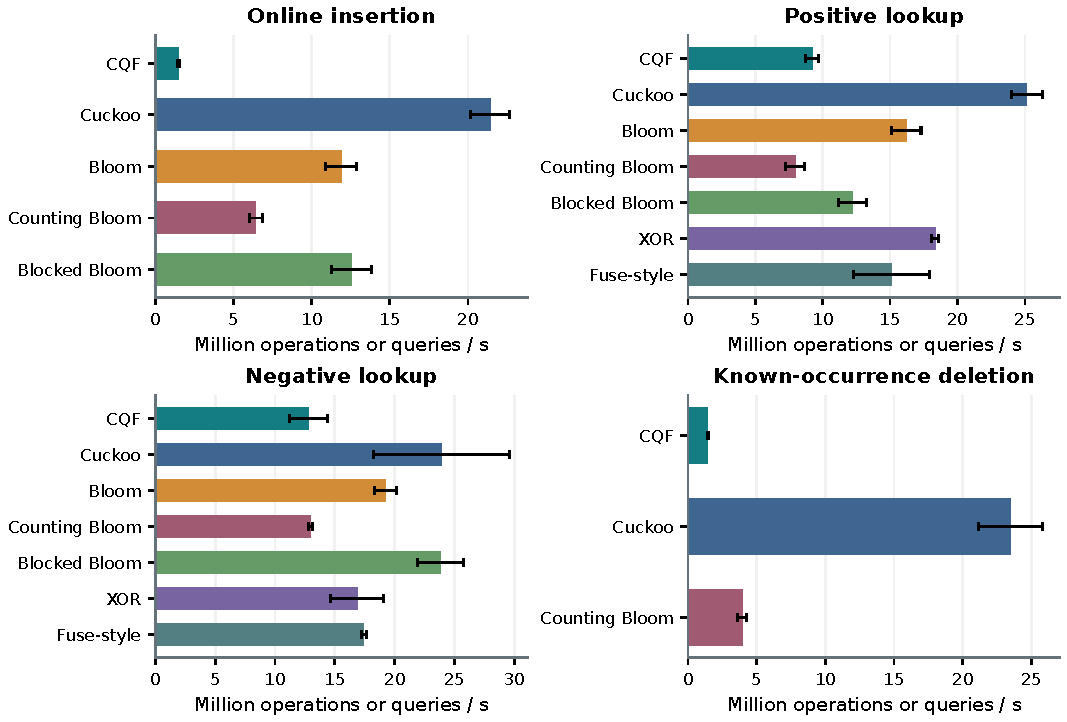
\includegraphics[width=\linewidth]{uniform_operations.pdf}
\caption{Supported operations on the 67M uniform stream. Bars show mean throughput and whiskers show one sample SD across three runs. Static filters appear in query panels only. The relative ranking is specific to these implementations and this translated execution environment.}
\label{fig:uniform}
\end{figure}

At this scale, \UniformFastestQuery{} reaches \UniformFastestQueryRate{}\,million successful queries per second. CQF achieves \CqfPositiveUniformLarge{}\Mops{} for the same query class and \CqfNegativeUniformLarge{}\Mops{} for negative queries. These results do not establish a universal advantage for one AMQ family: counting, deletion and immutable construction impose different costs, and the implementations use different hash and access paths.

The primary CQF occupies \PrimaryCqfMemory{}\,MB at about 50\% distinct load. It is therefore larger than the \BloomMemoryLarge{}\,MB Bloom filter, reversing the earlier report's three-filter space ordering. Equation~\ref{eq:cqf-sizing} explains the reversal: the allocation doubles when the workload crosses a power-of-two capacity boundary. CQF's occupied-slot count after insertion is \UniformOccupiedLarge{}, whereas its number of stored fingerprints is \UniformStoredLarge{}; colliding keys can share a fingerprint counter.
\finding{The large-scale comparison changes the space story as well as the speed story. A near-full CQF and a half-full CQF are different operating points.}
\clearpage
